\begin{Exercise}[title=Courbure de fibre optique]
Une fibre optique est constitué d'une âme en verre d'indice $n_1$=1,66 et de diamètre $d$ = \SI{0.05}{\mm} entourée d'une gaine en verre d'indice $n_2$=1,52. on courbe la fibre éclairée sous incidence normale.
%\begin{figure}[h!]
\begin{center}
  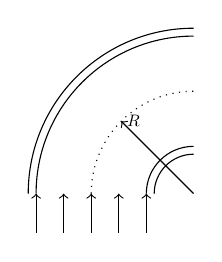
\begin{tikzpicture}[scale=0.5]
    \draw (-1,0) arc (180:90:1);
    \draw (-1.2,0) arc (180:90:1.2);
    \draw (-2.6,0)[dotted] arc (180:90:2.6);
    \draw (-4,0) arc (180:90:4);
    \draw (-4.2,0) arc (180:90:4.2);
    \draw (0,0)[->] --  (135:2.6) node[right,scale=0.6]{$R$};

    \draw (-4.0,-1)[->]-- (-4.0,0);
    \draw (-3.3,-1)[->]-- (-3.3,0);
    \draw (-2.6,-1)[->]-- (-2.6,0);
    \draw (-1.9,-1)[->]-- (-1.9,0);
    \draw (-1.2,-1)[->]-- (-1.2,0);
  \end{tikzpicture}
\end{center}
%\end{figure}
\Question Quel est le rayon de courbure $R$ minimal pour lequel toute la lumière incidente traverse la fibre?
\end{Exercise}
\begin{Answer}
en partant de $\sin(i) = \frac{n_2}{n_1}$ ( condition reflexion totale)
il faut $R > \frac{d}{2}\frac{n_1+n_2}{n_1-n_2}$
\begin{center}
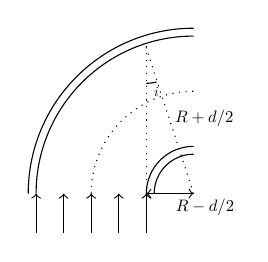
\begin{tikzpicture}[scale=0.5]
\draw (-1,0) arc (180:90:1);
\draw (-1.2,0) arc (180:90:1.2);
\draw (-2.6,0)[dotted] arc (180:90:2.6);
\draw (-4,0) arc (180:90:4);
\draw (-4.2,0) arc (180:90:4.2);
\draw (-4.0,-1)[->]-- (-4.0,0);
\draw (-3.3,-1)[->]-- (-3.3,0);
\draw (-2.6,-1)[->]-- (-2.6,0);
\draw (-1.9,-1)[->]-- (-1.9,0);
\draw (-1.2,-1)[->]-- (-1.2,0);

\draw (-1.2,0)[dotted] -- (-1.2,3.88);
\draw (0,0)[dotted] -- node[right,scale=0.6]{$R+d/2$} (108:4);
\draw (0,0)[<->] -- node[below right,scale=0.6]{$R-d/2$}(-1.2,0);
\draw (-1.2,2.8) arc(-90:-75:1) node[below,scale=0.5]{$i$};
\end{tikzpicture}
\end{center}
\end{Answer}
